\documentclass{article}

\usepackage{graphicx}
\usepackage{float}
\usepackage{fancyhdr}
\usepackage{mathtools}

\pagestyle{fancy}

\lhead{Robin Touche 900610-3270}
\rhead{robint@student.chalmers.se}

\begin{document}
\setcounter{section}{1}
\chapter{Homework 0}
\subsection{}

Bayes' rule states that $P(A\mid B) = \frac{P(A)P(B\mid A)}{P(B)}$. Let A be the
probability of me having cancer and let B be the probability of me testing
positive.

So to calcuate the probability of me having cancer given that I test positive
($P(A\mid B)$) we must calculate $P(A)$, $P(B\mid A)$ and $P(B)$.  We know
$P(A)$ (me having cancer) and $P(B\mid A)$ (me testing positive given that I
do, in fact, have cancer) from the assignment. 0.0001 and 0.99 respectively.

To calculate $P(B)$ we take the probability of testing positive times the
probability of having cancer plus the probability of me testing a false
positive. We can add these probabilities since we know that the events are
totally disjunct (I can't both have cancer and not have it).

\begin{equation}
0.99 \cdot 0.0001 + 0.01 \cdot 0.9999 = 0.0100989
\end{equation}

So the final probability becomes:

\begin{equation}
  P(A\mid B) = \frac{P(A)P(B\mid A)}{P(B)} =
  \frac{0.0001 \cdot 0.99}{0.0100989} \approx 0.0098 \approx 1\%
\end{equation}

\subsection{}

The covariance $cov(X,Y) = \mathbf{E}[(X - \mathbf{E}[X])(Y - \mathbf{E}[Y])]$
of $x$ and $y$ can be simplified to $\mathbf{E}[XY] -
\mathbf{E}[X]\mathbf{E}[Y]$ where $\mathbf{E}[X]$ is the expected value of $X$.

By definition the expected value of a continous random variable is calculated as

\begin{equation}
  \label{expvalue}
  \mathbf{E}[X] = \int_{-\infty}^{\infty} x f(x) dx
\end{equation}

where $f(x)$ is the probability density function. Since we know that $X$ is
uniformly distribuited in this interval the density function is just a constant
we can move outside the integral and the entire equation becomes

\begin{equation}
  \mathbf{E}[X] = c \int_{-\infty}^{\infty} x dx
\end{equation}

wich we know to be $0$. This means that we do not need to calculate the
expected value of $Y$ since $\mathbf{E}[X]\mathbf{E}[Y] = 0$. This, in turn,
means that to get a covariance of $0$ we need to prove that $\mathbf{E}[XY] =
0$ as well.

We know that $Y = X^2$ so $XY = X^3$. This means that we need to calculate
$\mathbf{E}[X^3]$. Using equation \ref{expvalue} we get that the expected value
of $X^3$ is also $0$.

\setcounter{section}{2}
\subsection{}

\begin{figure}[H]
\centering
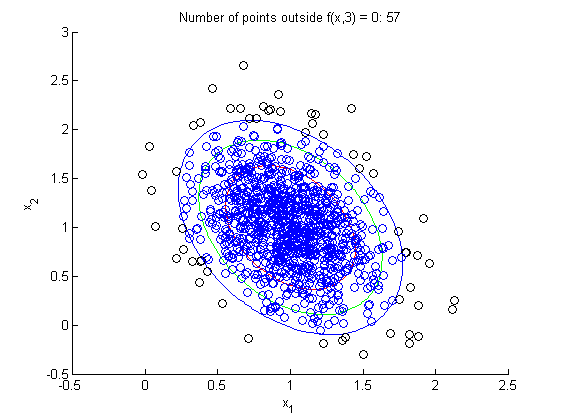
\includegraphics[scale=0.7]{fig21.png}
\end{figure}

Note that Matlab only seems to draw the plots when it wants to. I had to
restart my Matlab a couple of times.

\subsection{}

\begin{figure}[H]
\centering
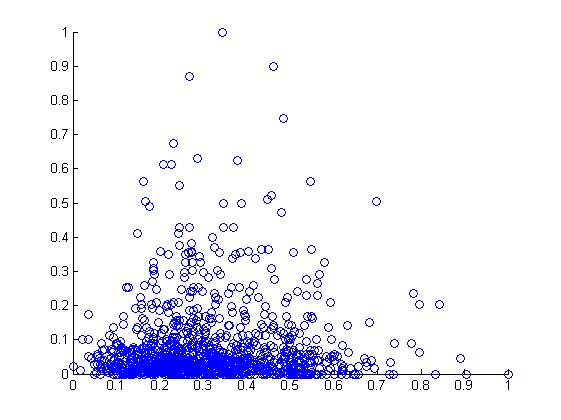
\includegraphics[scale=0.7]{fig22.png}
\end{figure}

Correlation coefficients are a normalised version of the covariance and $Y$ is
a normalised version of $X$ the correlation matrix of $Y$ is identical to that
of $X$.

The plot shows that the two features with the samllest correlation does,
indeed, have little correlation.

\end{document}
